\documentclass[12pt]{article}
\usepackage{hyperref}
\hypersetup{setpagesize=false,unicode,pdfborder=0 0 0}
 \ifx\pdfhorigin\undefined%
\usepackage[3D,dvipdfmx]{movie15}
\else%
\usepackage[3D]{movie15}
\fi%
\FPmessagesfalse%
 \usepackage{bm}
\def\V#1{\bm{#1}}
\def\ASYprefix{}
\newbox\ASYbox
\newdimen\ASYdimen
\long\def\ASYbase#1#2{\leavevmode\setbox\ASYbox=\hbox{#1}\ASYdimen=\ht\ASYbox%
\setbox\ASYbox=\hbox{#2}\lower\ASYdimen\box\ASYbox}
\long\def\ASYaligned(#1,#2)(#3,#4)#5#6#7{\leavevmode%
\setbox\ASYbox=\hbox{#7}%
\setbox\ASYbox\hbox{\ASYdimen=\ht\ASYbox%
\advance\ASYdimen by\dp\ASYbox\kern#3\wd\ASYbox\raise#4\ASYdimen\box\ASYbox}%
\put(#1,#2){#5\wd\ASYbox 0pt\dp\ASYbox 0pt\ht\ASYbox 0pt\box\ASYbox#6}}%
\long\def\ASYalignT(#1,#2)(#3,#4)#5#6{%
\ASYaligned(#1,#2)(#3,#4){%
\special{ps:gsave currentpoint currentpoint translate [#5 0 0] concat neg exch neg exch translate}%
}{%
\special{ps:currentpoint grestore moveto}%
}{#6}}
\long\def\ASYalign(#1,#2)(#3,#4)#5{\ASYaligned(#1,#2)(#3,#4){}{}{#5}}
\def\ASYraw#1{
currentpoint currentpoint translate matrix currentmatrix
100 12 div -100 12 div scale
#1
setmatrix neg exch neg exch translate}
\usepackage{graphicx}
\makeatletter
\def\Ginclude@eps#1{%
 \message{<#1>}%
  \bgroup
  \def\@tempa{!}%
  \dimen@\Gin@req@width
  \dimen@ii.1bp%
  \divide\dimen@\dimen@ii
  \@tempdima\Gin@req@height
  \divide\@tempdima\dimen@ii
    \special{PSfile=#1\space
      llx=\Gin@llx\space
      lly=\Gin@lly\space
      urx=\Gin@urx\space
      ury=\Gin@ury\space
      \ifx\Gin@scalex\@tempa\else rwi=\number\dimen@\space\fi
      \ifx\Gin@scaley\@tempa\else rhi=\number\@tempdima\space\fi
      \ifGin@clip clip\fi}%
  \egroup}
\makeatother
\usepackage{color}
\setlength{\unitlength}{1pt}
\pagestyle{empty}
\textheight=138.646171bp
\textwidth=132.385827bp
\begin{document}
\makeatletter%
\let\ASYencoding\f@encoding%
\let\ASYfamily\f@family%
\let\ASYseries\f@series%
\let\ASYshape\f@shape%
\makeatother%
{\catcode`"=12%
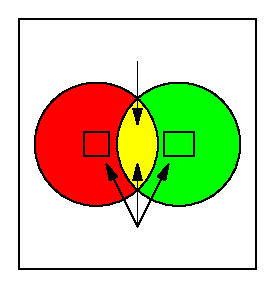
\includegraphics[bb=-57.192913 -60.323086 57.192913 60.323086]{latexusage-1_0.eps}%
}%
\kern -114.814774pt%
\special{ps:gsave}%
\begin{picture}( 114.814774, 121.098594)%
\special{ps:\ASYraw{
newpath 106.549213 60.323086 moveto
 106.549213 76.678324 93.290672 89.936865 76.935433 89.936865 curveto
 60.580194 89.936865 47.321654 76.678324 47.321654 60.323086 curveto
 47.321654 43.967847 60.580194 30.709306 76.935433 30.709306 curveto
 93.290672 30.709306 106.549213 43.967847 106.549213 60.323086 curveto
closepath
clip
}%
}%
\end{picture}%
\kern -114.814774pt%
\special{ps:grestore}%
\definecolor{ASYcolor}{gray}{0.000000}\color{ASYcolor}
\fontsize{12.000000}{14.400000}\selectfont
\usefont{\ASYencoding}{\ASYfamily}{\ASYseries}{\ASYshape}%
\ASYalign(37.590833,60.549297)(-0.500000,-0.500000){$A$}
\definecolor{ASYcolor}{gray}{0.000000}\color{ASYcolor}
\fontsize{12.000000}{14.400000}\selectfont
\ASYalign(77.223941,60.549297)(-0.500000,-0.500000){$\V{B}$}
\definecolor{ASYcolor}{gray}{0.000000}\color{ASYcolor}
\fontsize{12.000000}{14.400000}\selectfont
\ASYalign(57.407387,103.782406)(-0.500000,0.000000){$A\cap B$}
\definecolor{ASYcolor}{gray}{0.000000}\color{ASYcolor}
\fontsize{12.000000}{14.400000}\selectfont
\ASYalign(57.407387,17.316189)(-0.500000,-1.000000){$A\cup B$}
\end{document}
